%%%%%%%%%%%%%%%%%%%%%%%%%%%%%%%%%%%%%%%%%%%%%%%%%%%%%%%%%% 
\chapter{実行実験}\label{chap:experiment}
%%%%%%%%%%%%%%%%%%%%%%%%%%%%%%%%%%%%%%%%%%%%%%%%%%%%%%%%%% 

本章では,前章で提案した3つの符号化
\textsf{undirected},\textsf{directed},\textsf{acyclicity}
の性能を評価するために実行実験を行った.
%
実験に使用したベンチマーク問題集(計495問)は,以下の通りである.
\begin{itemize}
\item \textsf{color04} (計127問)\\
  グラフ彩色問題の国際競技会
  COLOR02/03/04~\footnote{\url{https://mat.tepper.cmu.edu/COLOR02/}}
  で使用された問題インスタンス.
\item \textsf{complete} (計15問)\\
  SATソルバーを用いた既存研究~\cite{soh14:jelia2014}で提供された
  完全グラフのインスタンス~\footnote{\url{https://tsoh.org/scarab/jelia2014/}}.
\item \textsf{knight} (計11問)\\
%  \cite{DBLP:conf/sat/EenS03}で用いられた
  $N\times N$の騎士巡回問題(Knight's Tour)のインスタンス.\\
  $N=8,12,20,30,40,50,60,70,80,90,100$の11通り.
\item \textsf{tsplib} (9問)\\
  巡回セールスマン問題のポータルサイトTSPLIBに公開されている
  インスタンス\footnote{\url{http://comopt.ifi.uni-heidelberg.de/software/TSPLIB95/hcp/}}.
\item \textsf{grid} (12問)\\
  $N$次の正方グリッドグラフのインスタンス($6\leq N\leq 17$).
\item \textsf{random} (320問)\\
  SATソルバーを用いた既存研究~\cite{soh14:jelia2014}で提供された
  ランダムグラフのインスタンス~\footnote{\url{https://tsoh.org/scarab/jelia2014/}}.
\item \textsf{usmap} (1問)\\
  図~\ref{fig:USmap}に示されたグラフ.
  D.~E~.Knuth の教科書
  The Art of Computer Programming~\cite{Knuth:TAOCP:SAT}
  に記載されている最短ハミルトン路問題の例.
\end{itemize}

使用した ASP システムは{\clingo}のバージョン5.4.0である.
実験環境は,Mac mini Intel Corei7 3.2GHz 64GBメモリである.

%%%%%%%%%%%%%%%%%%%%%%%%%%%%%%%%%%%%%%%%%%%%%%%%%%%%%%%%%%
\section{ハミルトン閉路問題の実験結果}
%%%%%%%%%%%%%%%%%%%%%%%%%%%%%%%%%%%%%%%%%%%%%%%%%%%%%%%%%%

%%%%%%%%%%%%%%%%%%%%%%%%%%%%%%%%%%%%%%%%%%%%%%%
\begin{table*}[t]\footnotesize
  \centering
% \tabcolsep = 0.8mm
% \renewcommand{\arraystretch}{1.2}
  \begin{tabular}{lr||r|r|r}
    頂点数 & 問題数 & \textsf{undirected} & \textsf{directed} & \textsf{acyclicity}\\
   \hline
    $\:\:\:\:\:\,\, 0 \leq |V| < 1000$  & 171   & 156   & \textbf{171}   & 155  \\
    $1000 \leq |V| < 2000$  & 165   & 120   & \textbf{158}   & 124  \\
    $2000 \leq |V| < 3000$  & 177   & 125   & \textbf{162}   & 73   \\
    $3000 \leq |V| < 4000$  & 185   & 104   & \textbf{148}   & 42   \\
    $4000 \leq |V| < 5000$  & 128   & 92    & \textbf{104}   & 28   \\
    $5000 \leq |V| < 6000$  & 80    & 63    & \textbf{68}    & 23   \\
    $6000 \leq |V| < 7000$  & 55    & 39    & \textbf{43}    & 21   \\
    $7000 \leq |V| < 8000$  & 28    & 12    & \textbf{14}    & 5    \\
    $8000 \leq |V| < 9000$  & 10    & 2     & \textbf{5}     & 1    \\
    $9000 \leq |V| < 10000$ & 2     & \textbf{2}     & \textbf{2}     & 1    \\
   \hline
    合計 & 1001 & 715   & \textbf{875}   & 473  
  \end{tabular}
  \vskip .5em
  \caption{ハミルトン閉路問題: 解けた問題数}
  \label{sat_table}
\end{table*}
%label{sat_table}
%%%%%%%%%%%%%%%%%%%%%%%%%%%%%%%%%%%%%%%%%%%%%%%

%%%%%%%%%%%%%%%%%%%%%%%%%%%%%%%%%%%%%%%%%%%%%%%
\begin{figure}[tb]
\begin{center}
  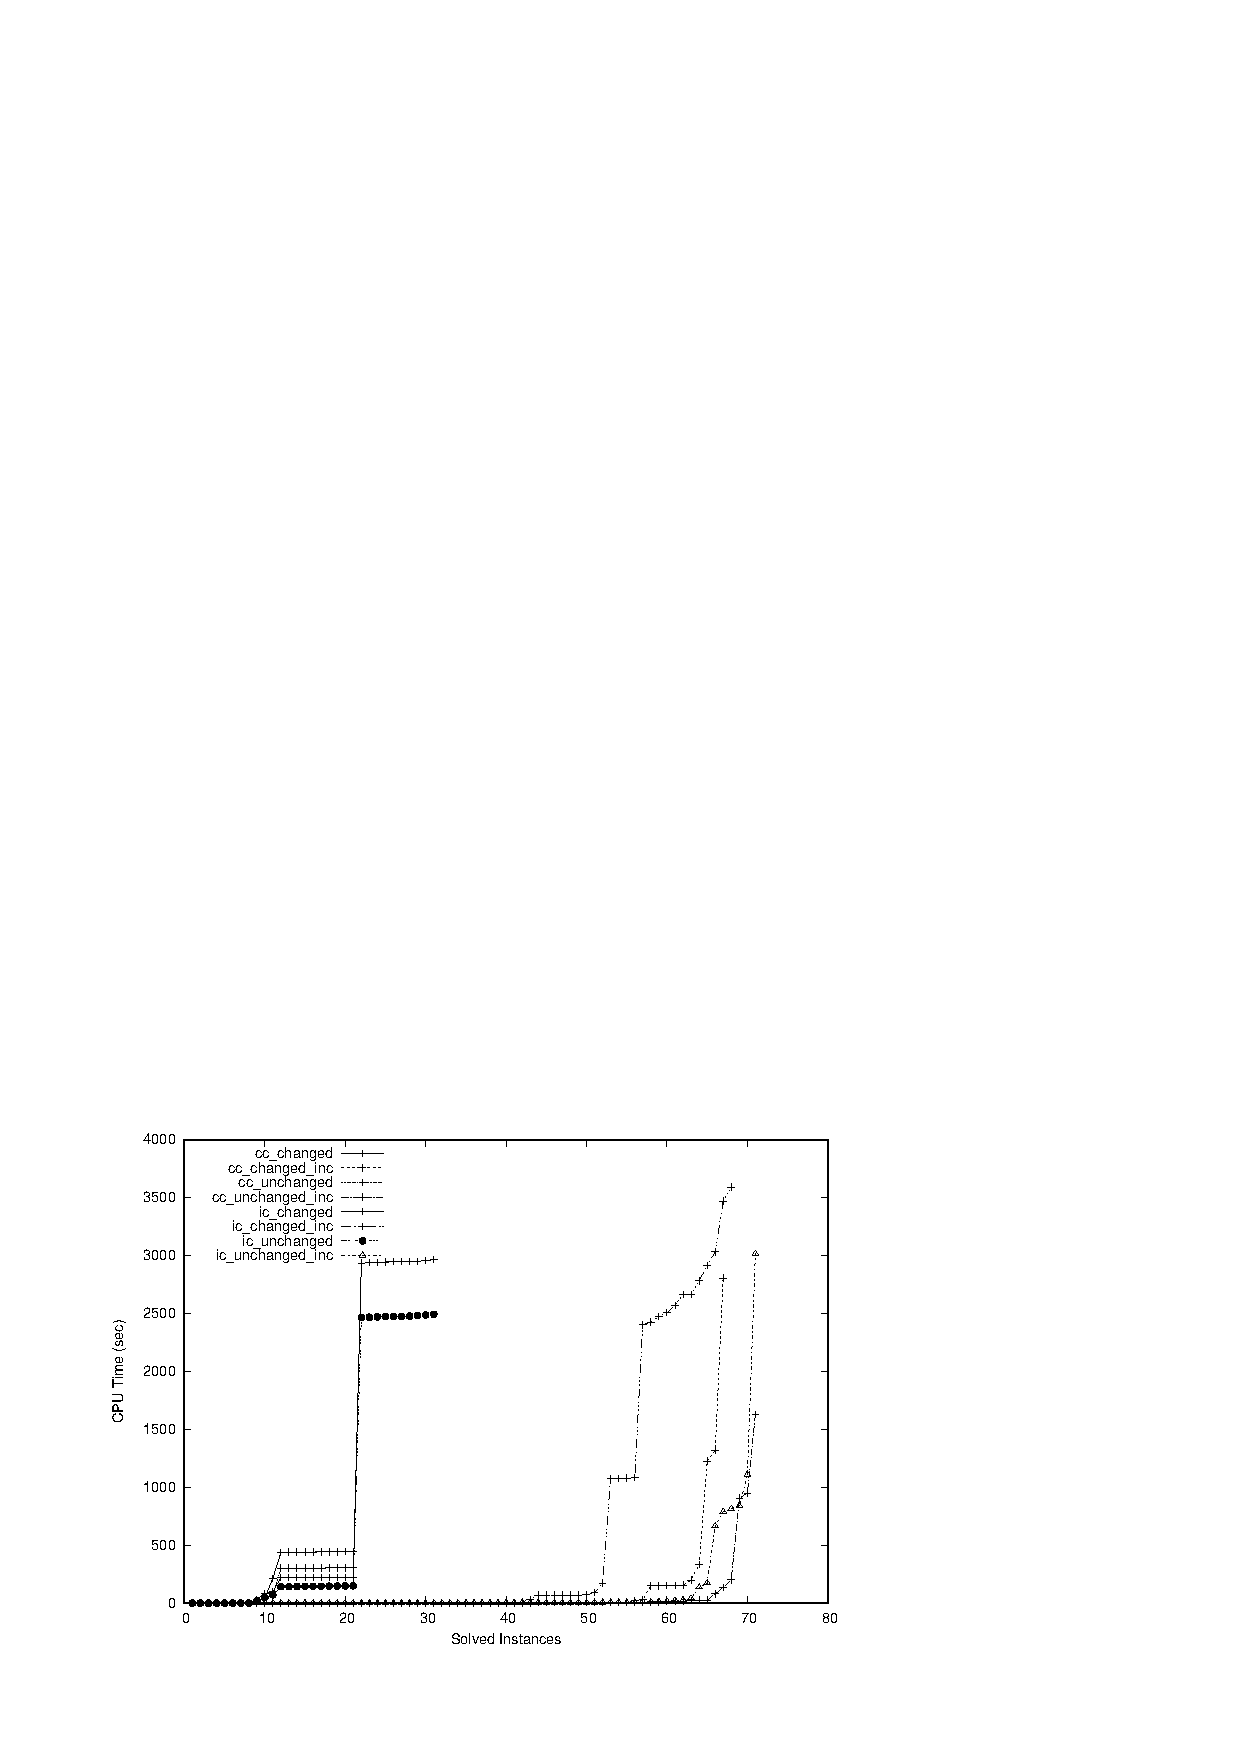
\includegraphics[width=0.6\linewidth]{fig/cactus.png}
\caption{ハミルトン閉路問題: カクタスプロット (\textsf{SAT+UNSAT})}
\label{cactus}
\end{center}
\end{figure}
%%%%%%%%%%%%%%%%%%%%%%%%%%%%%%%%%%%%%%%%%%%%%%%

%%%%%%%%%%%%%%%%%%%%%%%%%%%%%%%%%%%%%%%%%%%%%%%
\begin{figure}[tb]
\begin{center}
  \includegraphics[width=0.6\linewidth]{fig/cactussat.png}
\caption{ハミルトン閉路問題: カクタスプロット (\textsf{SAT})}
\label{cactussat}
\end{center}
\end{figure}
%%%%%%%%%%%%%%%%%%%%%%%%%%%%%%%%%%%%%%%%%%%%%%%

%%%%%%%%%%%%%%%%%%%%%%%%%%%%%%%%%%%%%%%%%%%%%%%
\begin{figure}[tb]
\begin{center}
\includegraphics[width=0.6\linewidth]{fig/cactusunsat.png}
\caption{ハミルトン閉路問題: カクタスプロット (\textsf{UNSAT})}
\label{cactusunsat}
\end{center}
\end{figure}
%%%%%%%%%%%%%%%%%%%%%%%%%%%%%%%%%%%%%%%%%%%%%%%

%--
オプションは\textit{trendy},一問あたりの時間制限を30分とした.
用いたベンチマーク問題は,\textsf{color04},\textsf{complete},\textsf{knight},\textsf{tsplib},\textsf{grid},\textsf{random}である.

%--
表~\ref{sat_table}に,各符号化で解けた問題数を示す.
ベンチマーク問題の種類ごとに,
\textsf{SAT},
\textsf{UNSAT},
\textsf{SAT+UNSAT}と解いた問題数を集計した.
\textsf{SAT+UNSAT}の問題数については,\textsf{undirected}符号化と\textsf{acyclicity}符号化が最大だった.
\textsf{SAT}の問題数については,\textsf{undirected}符号化が最大だった.
\textsf{UNSAT}の問題数については,\textsf{directed}符号化と\textsf{acyclicity}符号化が最大だった.

%--
図~\ref{cactus}に,\textsf{SAT+UNSAT}のカクタスプロットを示す.
縦軸は問題を解くのに要した CPU 時間,横軸は解けた問題数を表す.
グラフが右によるほど多くの問題を解けたことを示し,
下によるほどより速く解けたことを示す.
図~\ref{cactus}より,\textsf{acyclicity}符号化は,解けた問題数が同じ
\textsf{undirected}符号化と比較して,より高速に問題を説いていることが
確認できた.

%--
次に,図~\ref{cactussat}と図~\ref{cactusunsat}に,
\textsf{SAT}と\textsf{UNSAT}のカクタスプロットを示す.
図~\ref{cactussat}より,\textsf{SAT}のみの場合は,
\textsf{SAT+UNSAT}と比べて,符号化の優劣に差は見られなかった.
一方で,
図~\ref{cactusunsat}から,\textsf{UNSAT}のみの場合は,
\textsf{acyclicity}符号化と\textsf{undirected}符号化の優劣が逆転した.

%--
これらの結果から,
\textsf{SAT}な問題に対しては,解けた問題数と解くのに要したCPU時間
のどちらにおいても\textsf{acyclicity}符号化が優秀であったことがわかる.
一方で,\textsf{UNSAT}な問題に対しては,
解けた問題数では\textsf{directed}符号化と\textsf{acyclicity}が
解くのに要したCPU時間では\textsf{undirected}符号化が優秀であったことがわかる.

%--
表~\ref{sat_table}より,
\textsf{SAT+UNSAT}の問題数については,
\textsf{undirected}符号化と\textsf{acyclicity}符号化は同数だった.
しかし,その内訳には差があった.
結果に差があった問題は,\textsf{3-FullIns\_5}と\textsf{grid12}で,
それぞれ\textsf{color04}の\textsf{SAT}と,
\textsf{grid}の\textsf{UNSAT}に属する.
\textsf{3-FullIns\_5}は\textsf{undirected}に解けて
\textsf{acyclicity}に解けなかった.
一方で,\textsf{grid12}は,\textsf{acyclicity}に解けて
\textsf{undirected}に解けなかった.

\textsf{3-FullIns\_5}は\textsf{SAT}であったことから,
\textsf{undirected}符号化は\textsf{3-FullIns\_5}でハミルトン閉路を
偶然速く見つけられたと考える.
%% \textsf{color04}の他の問題を見ても,
%% \textsf{undirected}符号化が優秀であることを示してはいない.
%% 変数の数や制約の数も少なくない.
\textsf{grid12}については,変数の数や制約の数において,
\textsf{acyclicity}符号化が少ない値を示していたため,
要するCPUtimeを短縮できたと考える.

%% \textsf{grid12}は,\textsf{UNSAT}の問題に限定すれば
%% 要したCPU時間において優秀だった\textsf{undirected}符号化にのみ
%% 解けていなかった.
%% この問題の他にも,\textsf{grid}かつ\textsf{UNSAT}な問題を
%% 確認した.
%% \textsf{undirected}符号化がどの問題でも,
%% もっとも多く時間を要していた.
%% \textsf{undirected}符号化は\textsf{UNSAT}な\textsf{grid}問題が
%% 苦手であると考える.

%%%%%%%%%%%%%%%%%%%%%%%%%%%%%%%%%%%%%%%%%%%%%%%%%%%%%%%%%%
\section{最短ハミルトン閉路問題}
%%%%%%%%%%%%%%%%%%%%%%%%%%%%%%%%%%%%%%%%%%%%%%%%%%%%%%%%%%

%%%%%%%%%%%%%%%%%%%%%%%%%%%%%%%%%%%%%%%%%%%%%%%
\begin{table}[t]\footnotesize
  \caption{最短ハミルトン閉路問題: 得られた目的関数の値}
  \label{min_table_tr}
  \tabcolsep = 2mm
  %\renewcommand{\arraystretch}{1.0}
  \vskip .5em
  \centering
  \begin{tabular}{l|rrr}\hline
     問題 & \textsf{undirected} & \textsf{directed} & \textsf{acyclicity} \\
    \hline
    grid5&50,656*&50,656*&50,656* \\
    grid6&68,656*&68,656*&68,656* \\
    grid7&91,822*&91,822*&91,822* \\
    grid8&113,250&\textcolor{red}{112,916}&113,277 \\
    grid9&\textcolor{red}{142,502}&143,326&143,660 \\
    grid10&\textcolor{red}{172,703}&174,866&175,999 \\
    grid11&\textcolor{red}{200,399}&204,456&200,638 \\
    grid12&\textcolor{red}{231,278}&239,275&232,012 \\
    grid13&\textcolor{red}{276,692}&276,926&276,899 \\
    grid14&317,617&\textcolor{red}{317,144}&317,676 \\
    grid15&\textcolor{red}{375,906}&376,809&376,210 \\
    grid16&421,249&\textcolor{red}{419,737}&423,753 \\
    US48&11,698*&11,698*&11,698* \\
    \hline
    最適値と最良値の数 & 10 & 7 & 4\\    \hline
  \end{tabular}
\end{table}
%\label{min_table_tr}
%%%%%%%%%%%%%%%%%%%%%%%%%%%%%%%%%%%%%%%%%%%%%%%

%--
オプションは\textit{trendy},一問あたりの時間制限を3時間とした.
ベンチマーク問題として,\textsf{grid}と\textsf{usmap}を用いた.

%--
表\ref{min_table_tr}に,各符号化で
時間内に求められた最短距離を示す.
赤文字が,3符号化を比較した際の最良値である.
*マークは,時間内に最適解が求められたことを表している.
Bestは,符号化ごとに赤文字の個数を集計した値である.
Bestの値がもっとも大きかった\textsf{undirected}が優秀な性能を示した.

%%%%%%%%%%%%%%%%%%%%%%%%%%%%%%%%%%%%%%%%%%%%%%%%%%%%%%%%%%
\section{コスト制約付きハミルトン路問題}
%%%%%%%%%%%%%%%%%%%%%%%%%%%%%%%%%%%%%%%%%%%%%%%%%%%%%%%%%%

%%%%%%%%%%%%%%%%%%%%%%%%%%%%%%%%%%%%%%%%%%%%%%%
\begin{table}[htbp]
  \caption{実験結果3}
  \label{cost_table}
  \centering
  \begin{tabular}{|l|r|rrr|}
    \hline
    制約Cost値    &	Models & undirected & directed & acyclicity \\
    \hline
    11698   &	1      &\textcolor{red}{2.919} &10.020 & 4.355	\\
    11814   &	8      &5.458  &7.416	& \textcolor{red}{4.136}	\\
    11931   &	28     &\textcolor{red}{3.226}&10.317	& 4.799	\\
    12282   &	388    &\textcolor{red}{9.993}&15.787	& 10.715	\\
    12867   &	16180  &16.386       &23.406	& \textcolor{red}{10.819}\\
    14037   &	939209 &47.894       &41.515	& \textcolor{red}{24.655}\\
    15207   &	4525541&85.256       &56.953	& \textcolor{red}{41.217}\\
    16377   &	6702964&93.595       &51.991	& \textcolor{red}{41.301}	\\
    17547   &	6876526&91.750       &46.065	& \textcolor{red}{37.290}	\\
    18716   &	6876928&95.659       &45.416	& \textcolor{red}{37.905}	\\
    \hline
    Average &   & 45.2136 & 30.889  & \textcolor{red}{21.7192}\\
    Best    &   & 3 & 0 & \textcolor{red}{7} \\
    \hline
  \end{tabular}
\end{table}
%\label{cost_table}
%%%%%%%%%%%%%%%%%%%%%%%%%%%%%%%%%%%%%%%%%%%%%%%

%--
オプションは\textit{crafty},一問あたりの時間制限を3時間とした.
ベンチマーク問題として\textsf{usmap}を用いた.
閾値は表\ref{cost_table}にあるように11698〜18716までの10の値を与えた.

%--
表~\ref{cost_table}に閾値ごとの解の個数と
各符号化が要したCPU時間をまとめた.
赤文字が3符号化の中での最短時間を表している.
Averageは,各符号化のCPU時間の平均値を示す.
Bestは,各符号化ごとの赤文字の個数を示す.

%--
Bestより,10の閾値の内の7つにて\textsf{acyclicity}が最短時間で解いている.
Averageでも,\textsf{acyclicity}が最小である.
以上より,\textsf{acyclicity}がもっとも優秀であった.
%%%%%%%%%%%%%%%%%%%%%%%%%%%%%%%%%%%%%%%%%%%%%%%%%%%%%%%%%%

%%% Local Variables:
%%% mode: latex
%%% TeX-master: "paper"
%%% End:
